\subsection{Ablation Study}

\textcolor{red}{One of the ablation study is change the shift and rotation hyperparameter to show the performance with the two-session protocol on the deformable finger knuckle database \cite{fingerknuckledbv3.0}. We change the shift size from 0 to 8, and the rotation angle also from 0 to 8, and the interval value is 4. From the Figure \ref{ablation-study}, we can get from the ROC and CMC }

\begin{figure}[H]
    \centering
    \begin{subfigure}[b]{0.45\linewidth}
        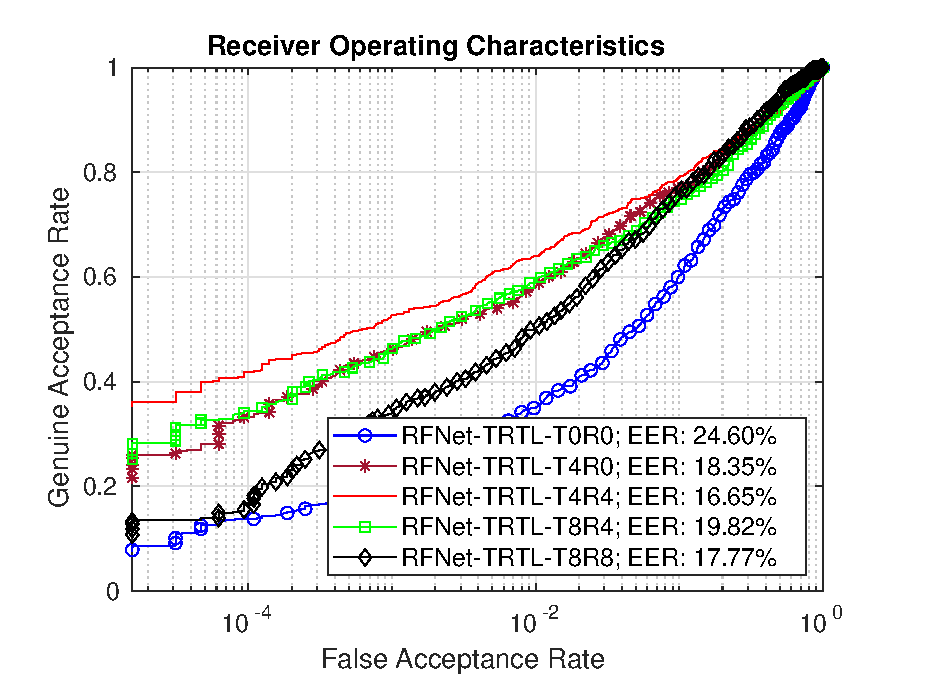
\includegraphics[width=\linewidth]{Figures/ablation-roc_compare_new.eps}
        \caption{}
    \end{subfigure}
    \begin{subfigure}[b]{0.45\linewidth}
        \includegraphics[width=\linewidth]{Figures/ablation-cmc_compare_new.eps}
        \caption{}
    \end{subfigure}
    \caption{Comparative ROC (a) and corresponding CMC (b) for two-session of the Finger Knuckle Database (Version 3.0) \cite{fingerknuckledbv3.0}. For approving our TRTL loss function efficiency, we change the translation parameter and rotation parameter to show the different matching performance.}
    \label{ablation-study}
\end{figure}

\begin{figure}[H]
    \centering
    \begin{subfigure}[b]{0.45\linewidth}
        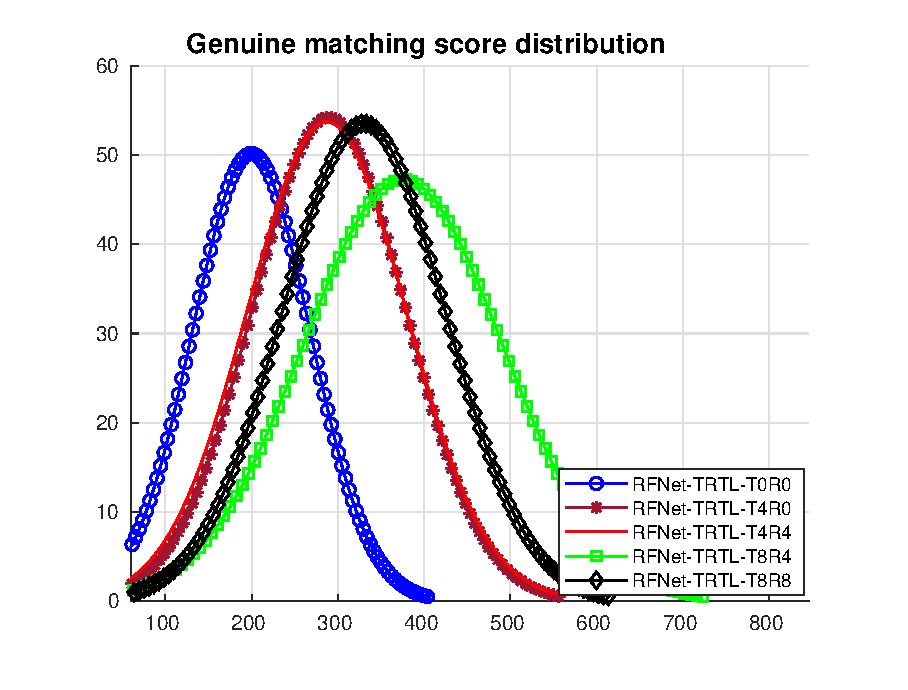
\includegraphics[width=\linewidth]{Figures/ablation-genuine_distribution.eps}
        \caption{}
    \end{subfigure}
    \begin{subfigure}[b]{0.45\linewidth}
        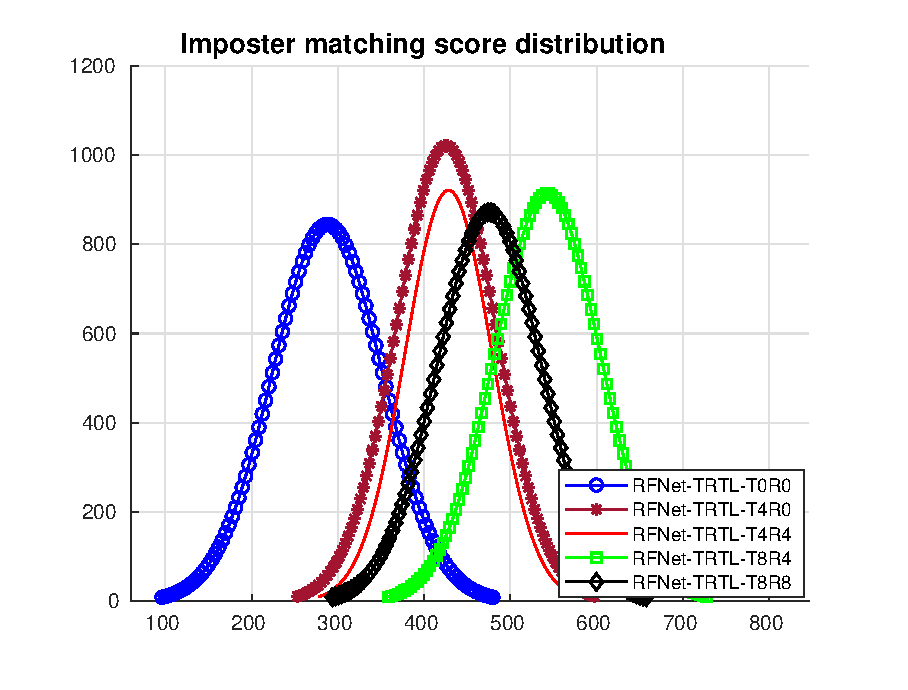
\includegraphics[width=\linewidth]{Figures/ablation-imposter_distribution.eps}
        \caption{}
    \end{subfigure}
    \caption{Genuine matching score distribution (a) and Imposter matching score (b) for two-session of the Finger Knuckle Database (Version 3.0) \cite{fingerknuckledbv3.0}. For approving our TRTL loss function efficiency, we change the translation parameter and rotation parameter to show the different matching performance.}
    \label{ablation-study-distribution}
\end{figure}


\textcolor{red}{The other ablation study is change the input image size. From segmented finger knuckle by YOLOv5x-CSL, the minimal size of ROI is about $189*224$. Therefore, we keep the same ratio to change all segmented finger knuckle to $184*208$ due to rectangle bounding boxes. And in this kind of situation, we change the vertical and horizontal size with different size. And we make the vertical shifting size bigger than horizontal shifting size, get the result in the Figure \ref{ablation-study-rectangle}.}

\begin{figure}[H]
    \centering
    \begin{subfigure}[b]{0.45\linewidth}
        \includegraphics[width=\linewidth]{Figures/ablation-study-184-208/roc_compare_new.eps}
        \caption{}
    \end{subfigure}
    \begin{subfigure}[b]{0.45\linewidth}
        \includegraphics[width=\linewidth]{Figures/ablation-study-184-208/cmc_compare_new.eps}
        \caption{}
    \end{subfigure}
    \caption{}
    \label{ablation-study-rectangle}
\end{figure}


\textcolor{red}{Put the Grad-CAM to show neural network output feature from the original input picture.}
........